% !TeX spellcheck = <english>
\documentclass{beamer}
%\documentclass[aspectratio=169]{beamer}

% You have to install the theme first!

% corporate design of TU Wien
\usetheme[font=futura]{tuw}

% background "TU main building" on title page
%\usetheme[tuw_background]{tuw}
% individual background on title page
%\usetheme[tuw_image=TU_Background]{tuw}
% white logo if you have a dark background image
%\usetheme[tuw_image=TU_Background,tuw_whitelogo]{tuw}
% sidebar (not in TU Wien CD! but nice for long presentations)
% width of the sidebar can be changed with option: "width=2cm"
%\usetheme[outer=sidebar]{tuw}
% move frametitle up (beside logo)
%\usetheme[tuw_frametitletotop]{tuw}

% if you use german umlaute use T1 encoding:
%\usepackage[T1]{fontenc}
% default Latex fonts are not T1 supported -> bitmaps used, this is not nice on
% screen; you can use the lmodern package instead
%\usepackage{lmodern}
\usepackage[utf8]{inputenc}
\usepackage{listings}
\usepackage{booktabs}
\usepackage{url}
\usepackage{apacite}
\usepackage{tikz,pgfplots}
\usepackage{mathtools}

\pgfplotsset{compat=1.7}
\bibliographystyle{apacite}
\DeclarePairedDelimiter\norm{\lVert}{\rVert}
\setbeamertemplate{caption}[numbered]

%%% title page settings
\title[Buffering Station]{%
  Buffer Station
}
\subtitle{Information Technology in Automation}
\author{Philipp-Alexander Auer}
\date{\today}


%%% slides start here
\begin{document}

% first frame must include the title page!
\begin{frame}
  \titlepage
\end{frame}

% table of contents if you have a long presentation (uses 'part' and 'section'
% elements)
\begin{frame}{Outline}
  \tableofcontents
\end{frame}

\section{Station Five}

\subsection[Overview]{Overview}
\begin{frame}[fragile]
\frametitle{Station Five: Overview}
\begin{figure}
	\centering
	\scalebox{1}{
		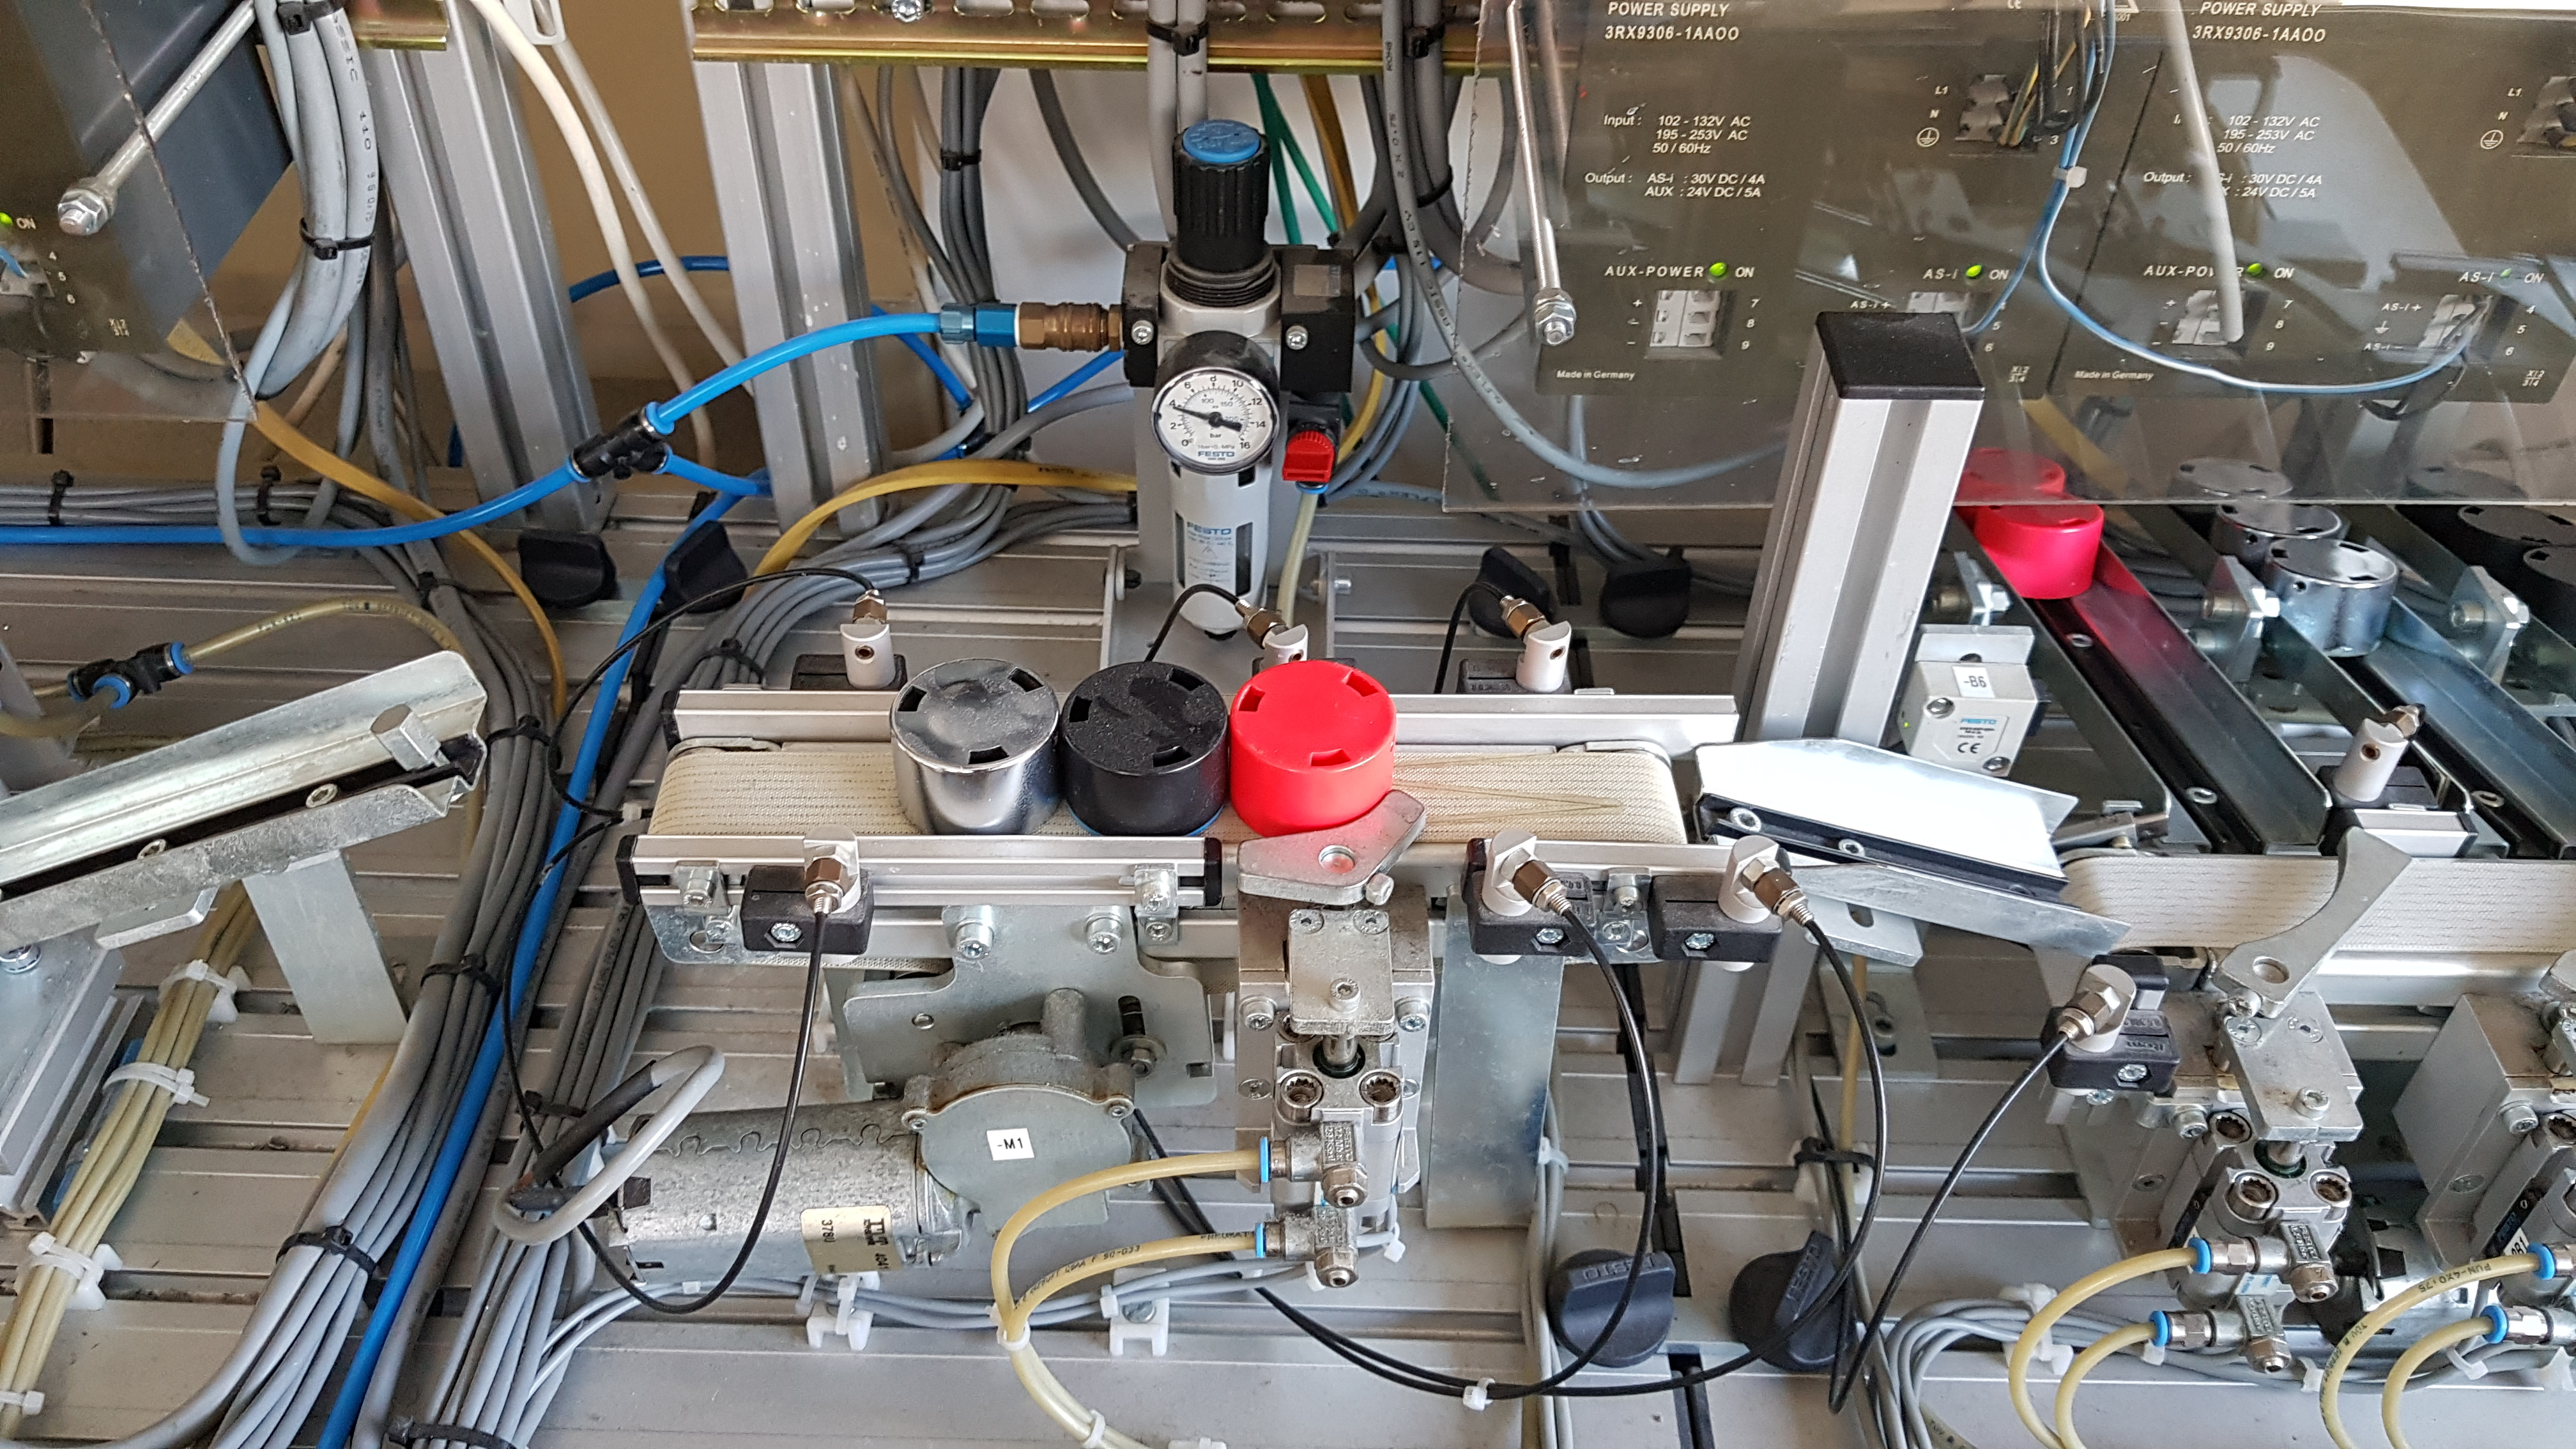
\includegraphics[width=\textwidth]{Photos/5_Station_4.jpg}
	}
	%\caption{Station 5 Part 1}
	\label{fig:stat54}
\end{figure}
\end{frame}

\begin{frame}[fragile]
\frametitle{Station Five: Overview}
\begin{figure}
	\centering
	\scalebox{1}{
		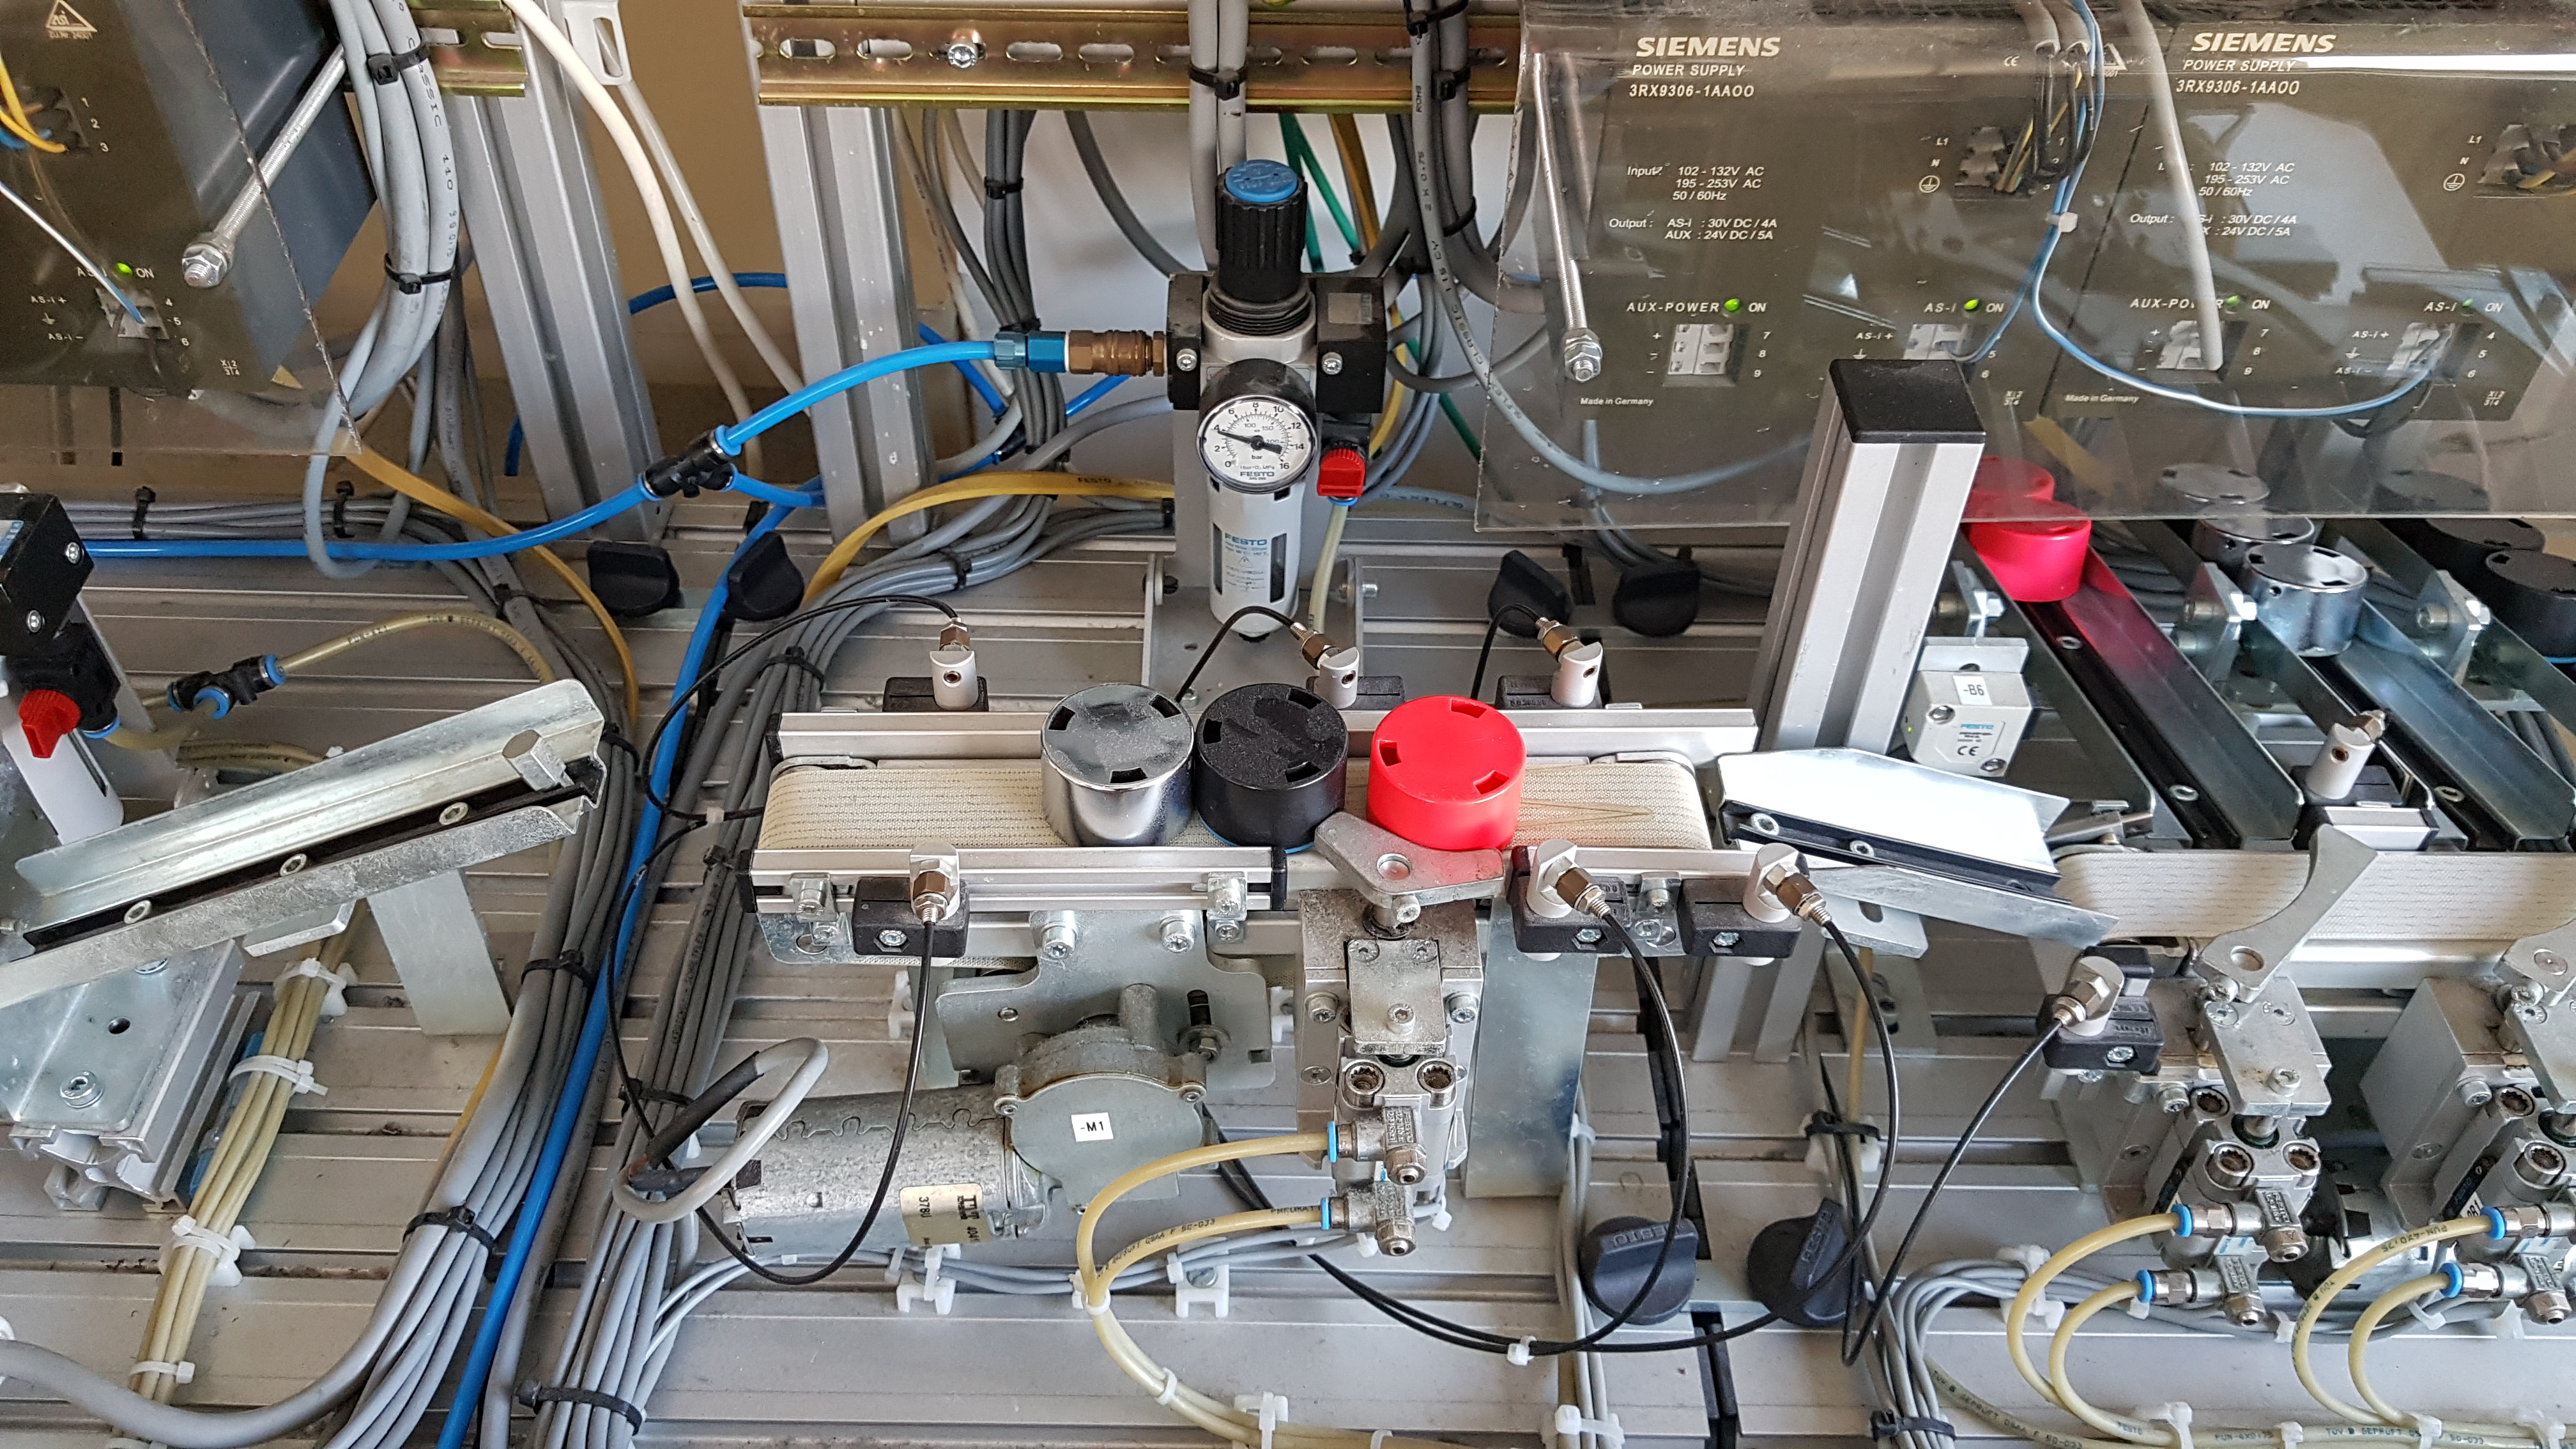
\includegraphics[width=\textwidth]{Photos/5_Station_5.jpg}
	}
	%\caption{Station 5 Part 1}
	\label{fig:stat55}
\end{figure}
\end{frame}

\begin{frame}[fragile]
\frametitle{Station Five: Overview}
\begin{figure}
	\centering
	\scalebox{1}{
		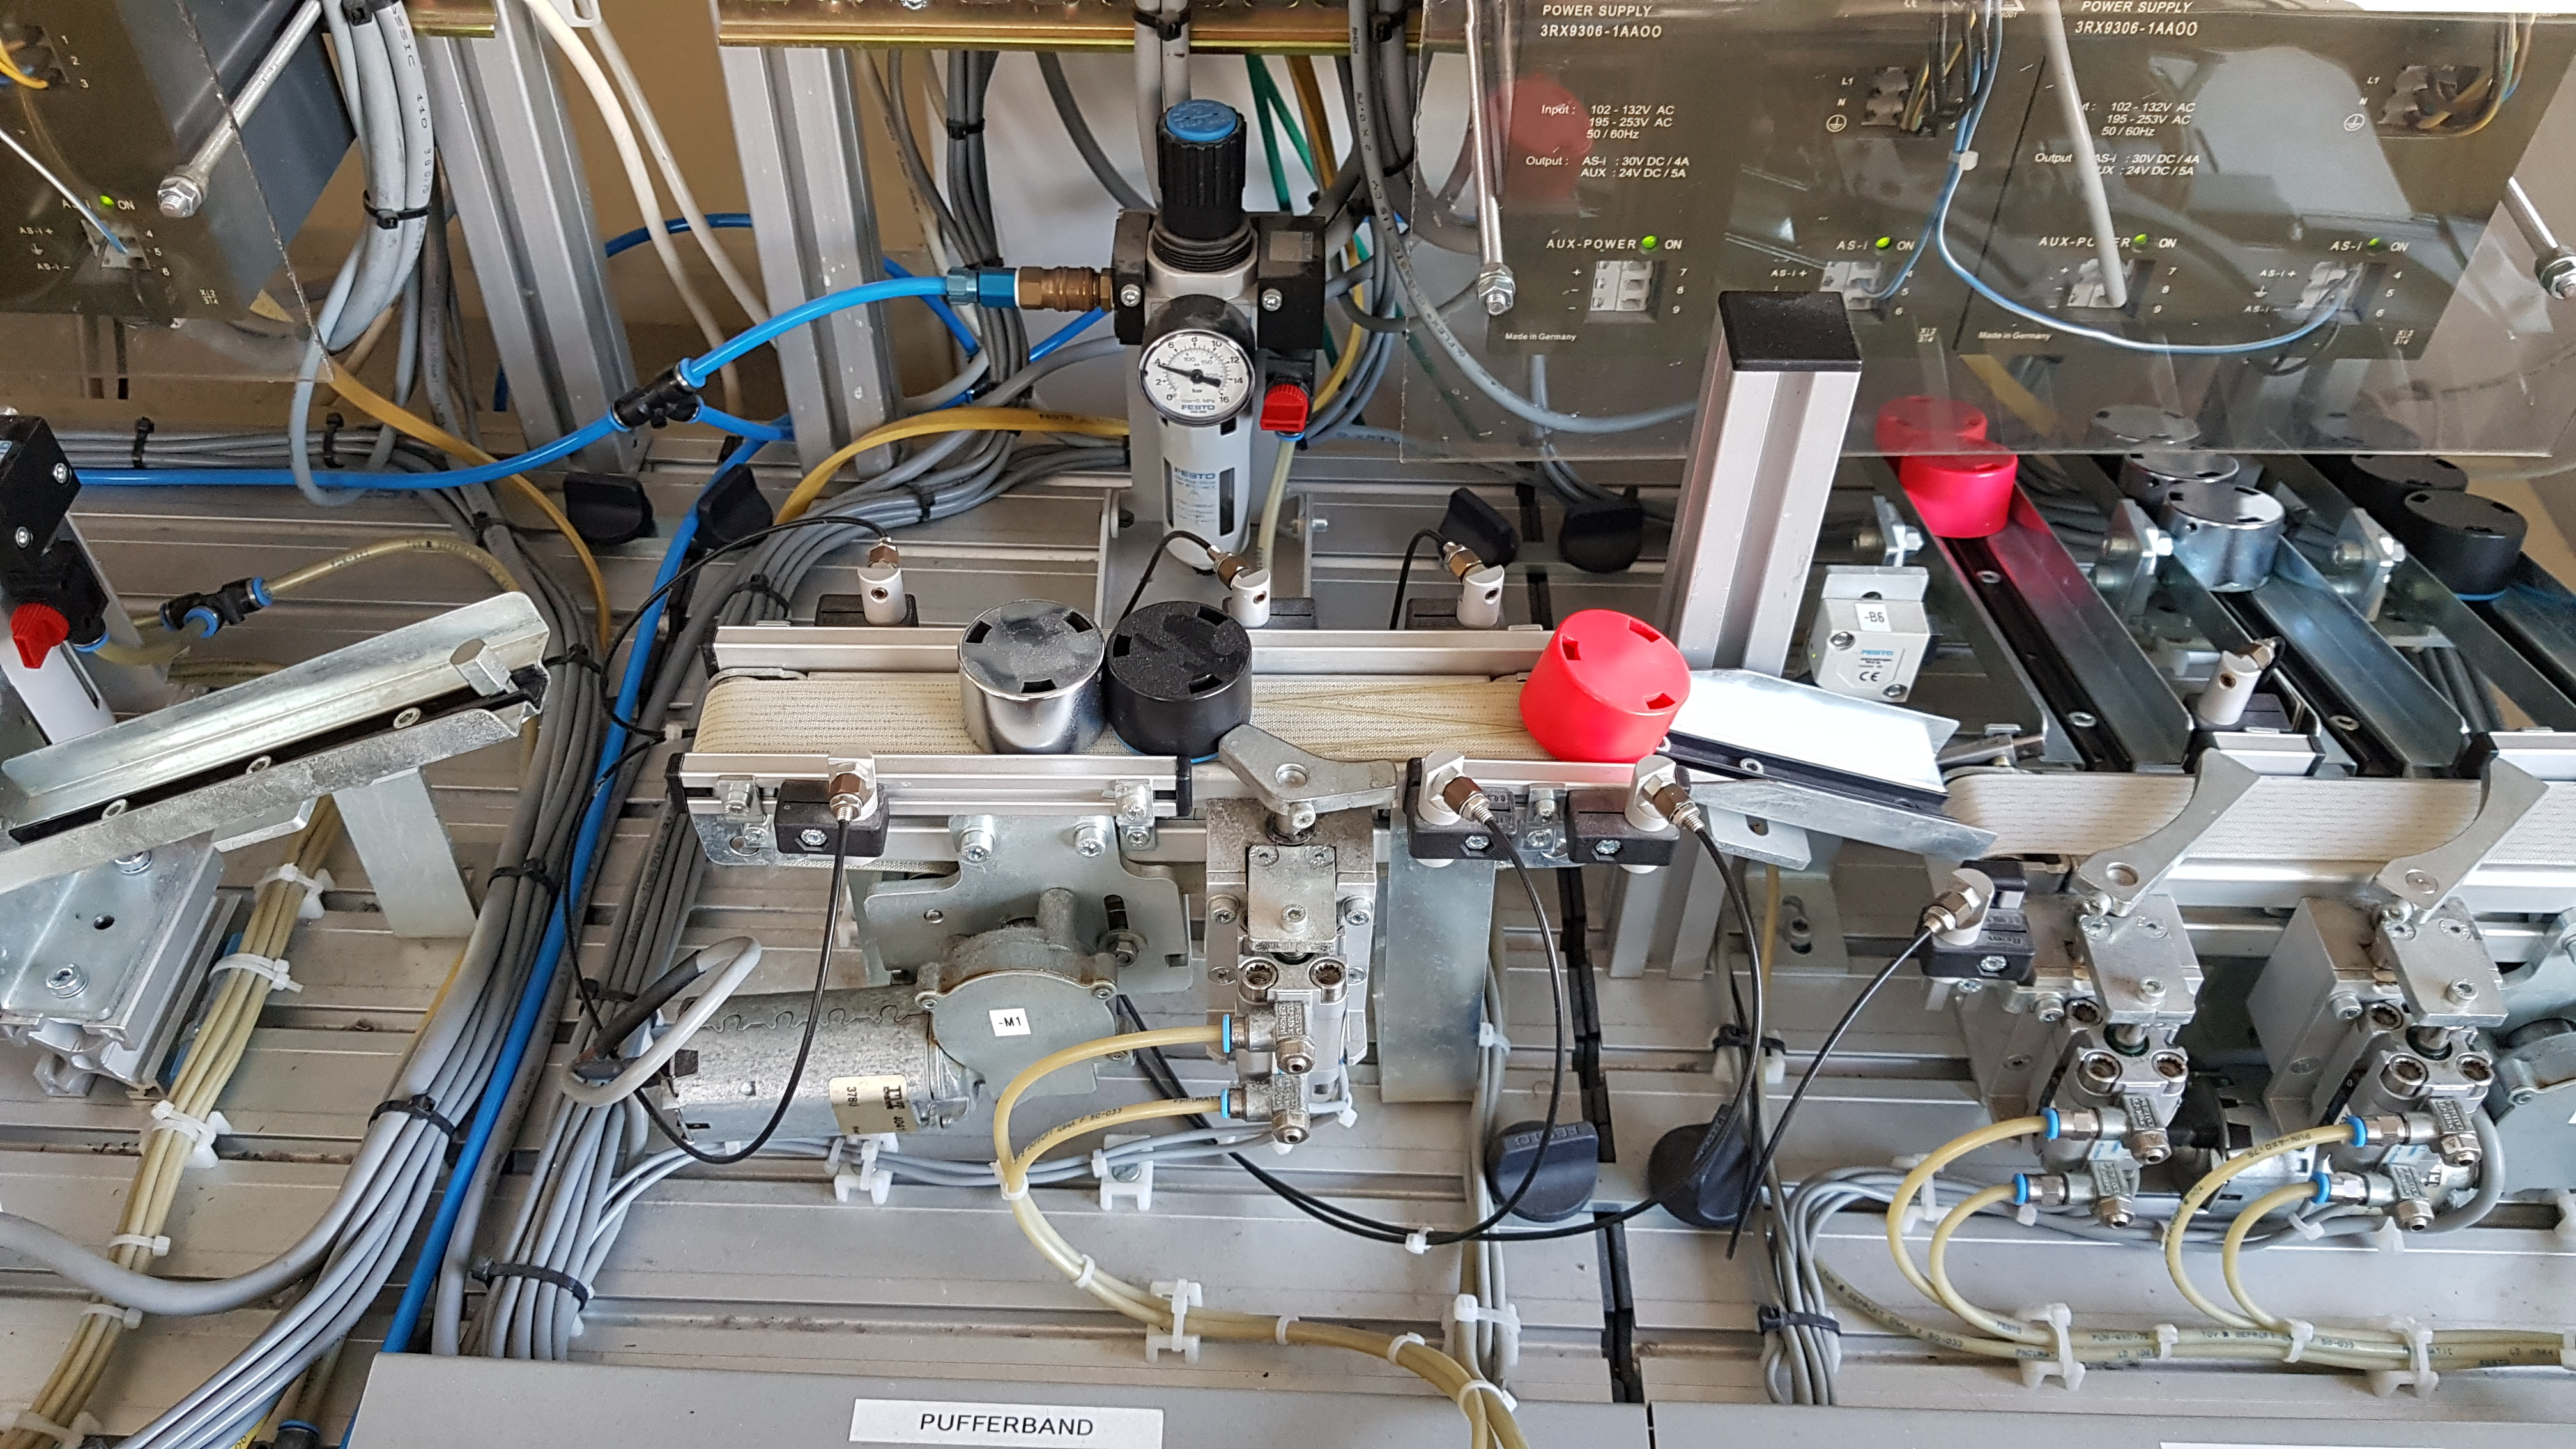
\includegraphics[width=\textwidth]{Photos/5_Station_6.jpg}
	}
	%\caption{Station 5 Part 1}
	\label{fig:stat56}
\end{figure}
\end{frame}
\section{SysML Model}
\subsection{Overview Package Diagram}
\begin{frame}[fragile]
\frametitle{Station Five: Overview}
\begin{figure}
	\centering
	\scalebox{0.65}{
		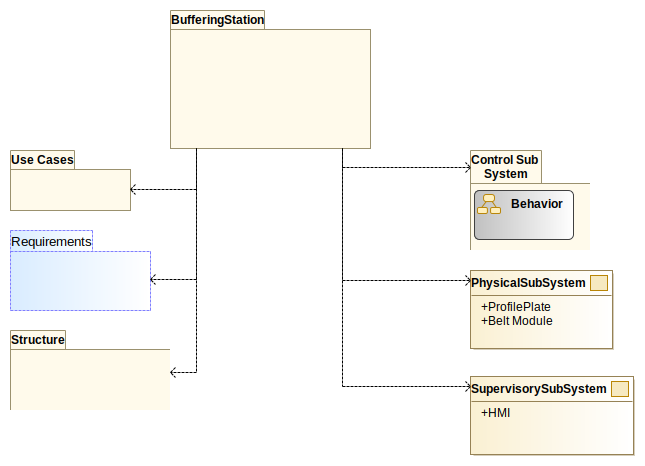
\includegraphics[width=\textwidth]{model-figures/overview.png}
	}
	\caption{Station 5: Overview Diagram}
	\label{dia:overview}
\end{figure}
\end{frame}
\subsection{Structure Diagram}
\begin{frame}[fragile]
\frametitle{Station Five: Structure}
\begin{figure}
	\centering
	\scalebox{0.65}{
		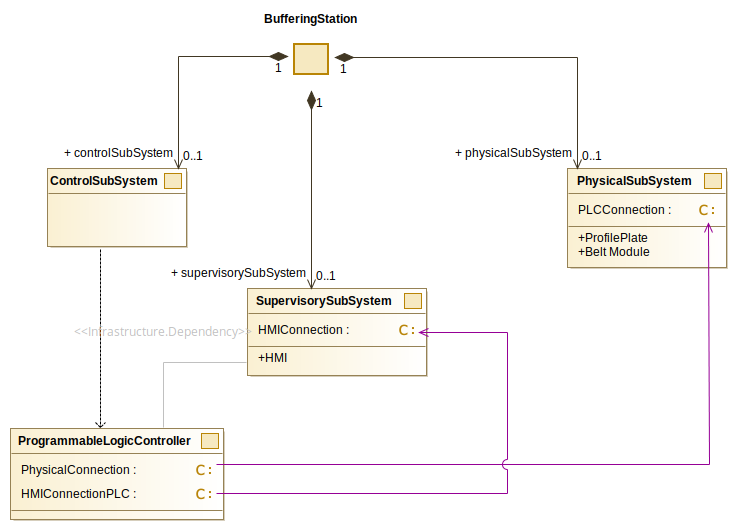
\includegraphics[width=\textwidth]{model-figures/structure.png}
	}
	\caption{Station 5: Structure Diagram}
	\label{dia:structure}
\end{figure}
\end{frame}

\subsection{Requirements Diagram}
\begin{frame}[fragile]
\frametitle{Station Five: Requirements}
\begin{figure}
	\centering
	\scalebox{1}{
		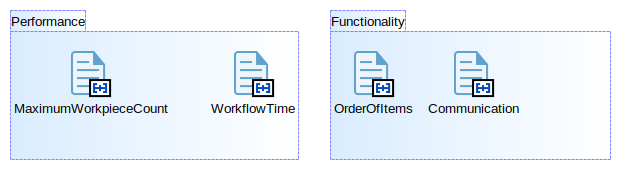
\includegraphics[width=\textwidth]{model-figures/requirements.png}
	}
	\caption{Station 5: Requirements Diagram}
	\label{dia:requirements}
\end{figure}
\end{frame}

\subsection{Use Cases Diagram}
\begin{frame}[fragile]
\frametitle{Station Five: Use Cases}
\begin{figure}
	\centering
	\scalebox{0.65}{
		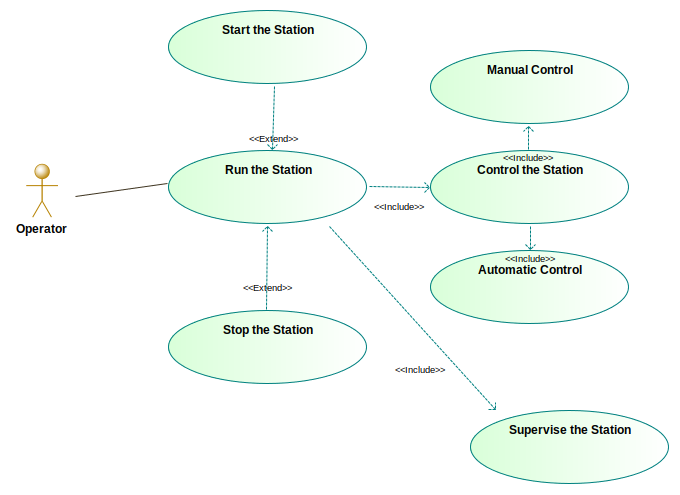
\includegraphics[width=\textwidth]{model-figures/usecase.png}
	}
	\caption{Station 5: Use Cases}
	\label{dia:usecase}
\end{figure}
\end{frame}

\subsection{Use Cases Diagram}
\begin{frame}[fragile]
\frametitle{Station Five: Behavior Diagram}
\begin{figure}
	\centering
	\scalebox{0.5}{
		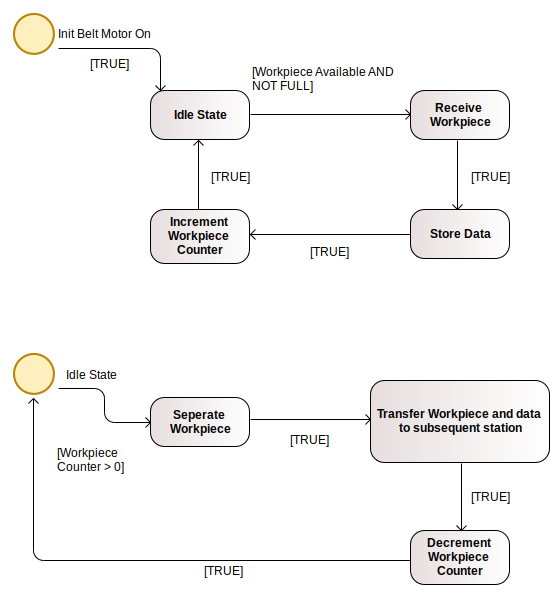
\includegraphics[width=\textwidth]{model-figures/control-beh.png}
	}
	\caption{Station 5: ControlSubSystem Behavior}
	\label{dia:behavior}
\end{figure}
\end{frame}


\subsection{PhysicalSubSystem}
\begin{frame}[fragile]
\frametitle{Station Five: PhysicalSubSystem}
\begin{figure}
	\centering
	\scalebox{1}{
		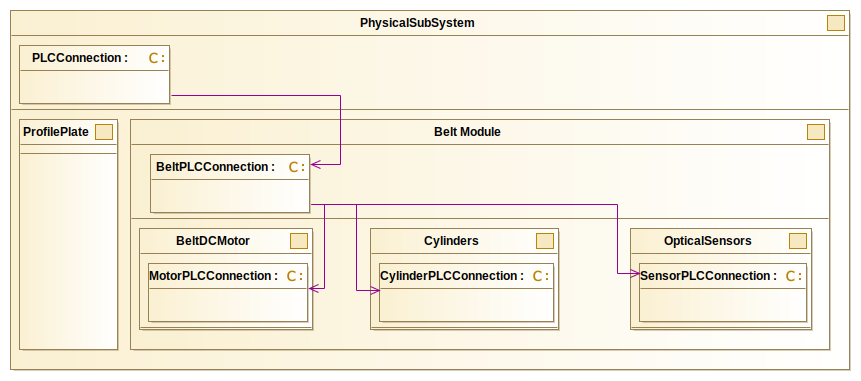
\includegraphics[width=\textwidth]{model-figures/physicalss.png}
	}
	\caption{Station 5: PhysicalSubSystem Block Diagram}
	\label{dia:physicalss}
\end{figure}
\end{frame}

\subsection{Miscellaneous}
\begin{frame}
\frametitle{Station Five: Miscellaneous}
	\begin{itemize}
		\item The SupervisorySubSystem models a very high-level abstraction of the \textbf{H}uman \textbf{M}achine \textbf{I}nterface.
		\item The \textbf{P}rogrammable \textbf{L}ogic \textbf{C}ontroller models a very high-level abstraction of the PLC we are using, just to emphasize its connections with the physical world
		\item The abstract connections shall emphasize the real-world physical connections (Profibus)
	\end{itemize}
\end{frame}
\end{document}
